\chapter{Despliegue del sistema en instancia EC2}
\label{AppendixG}

%%%%%%%%%%%%%%%%%%%%%%%%%%%%%%%%%%%%%%%%%%%%%%%%%%%%%%%%%%%%%%%%%%%%%%%%%%%%%
% parámetros para configurar el formato del código en los entornos lstlisting
%%%%%%%%%%%%%%%%%%%%%%%%%%%%%%%%%%%%%%%%%%%%%%%%%%%%%%%%%%%%%%%%%%%%%%%%%%%%%
\lstset{ %
    backgroundcolor=\color{white},   % choose the background color; you must add \usepackage{color} or \usepackage{xcolor}
    basicstyle=\footnotesize,        % the size of the fonts that are used for the code
    breakatwhitespace=false,         % sets if automatic breaks should only happen at whitespace
    breaklines=true,                 % sets automatic line breaking
    captionpos=b,                    % sets the caption-position to bottom
    commentstyle=\color{mygreen},    % comment style
    deletekeywords={...},            % if you want to delete keywords from the given language
    %escapeinside={\%*}{*)},          % if you want to add LaTeX within your code
    %extendedchars=true,              % lets you use non-ASCII characters; for 8-bits encodings only, does not work with UTF-8
    %frame=single,	                % adds a frame around the code
    keepspaces=true, keywordstyle=\color{blue}, language=[ANSI]C, % keeps spaces in text, useful for keeping indentation of code (possibly needs columns=flexible)% keyword style% the language of the code
    %otherkeywords={*,...},           % if you want to add more keywords to the set
    numbers=left, numbersep=5pt, numberstyle=\tiny\color{mygray},
    rulecolor=\color{black}, showspaces=false, showstringspaces=false,
    showtabs=false, stepnumber=1, stringstyle=\color{mymauve}, tabsize=2,
    title=\lstname, morecomment=[s]{/*}{*/} }% where to put the line-numbers; possible values are (none, left, right)% how far the line-numbers are from the code% the style that is used for the line-numbers% if not set, the frame-color may be changed on line-breaks within not-black text (e.g. comments (green here))% show spaces everywhere adding particular underscores; it overrides 'showstringspaces'% underline spaces within strings only% show tabs within strings adding particular underscores% the step between two line-numbers. If it's 1, each line will be numbered% string literal style% sets default tabsize to 2 spaces% show the filename of files included with \lstinputlisting; also try caption instead of title

\lstdefinelanguage{PythonUTF8}[]{Python}{
literate={á}{{\'a}}1 {é}{{\'e}}1 {í}{{\'i}}1 {ó}{{\'o}}1 {ú}{{\'u}}1
{Á}{{\'A}}1 {É}{{\'E}}1 {Í}{{\'I}}1 {Ó}{{\'O}}1 {Ú}{{\'U}}1
{ñ}{{\~n}}1 {Ñ}{{\~N}}1
}

\definecolor{mygreen}{rgb}{0,0.6,0}
\definecolor{mygray}{rgb}{0.5,0.5,0.5}
\definecolor{mymauve}{rgb}{0.58,0,0.82}

\section{Introducción}

El presente anexo documenta el procedimiento realizado para la instalación,
configuración y puesta en funcionamiento del entorno de servidor utilizado para
alojar la solución \texttt{EnviroSenseIoT}. Esta solución se desplegó sobre una
instancia virtual en Amazon EC2, se utilizaron servicios de infraestructura en
la nube para garantizar la disponibilidad, escalabilidad y acceso remoto seguro
al sistema.

Se detallan paso a paso las acciones ejecutadas para:
\begin{itemize}
    \item Crear una instancia EC2 en Amazon Web Services (AWS) con Ubuntu 24.04 con sus
          respectivas claves de acceso.
    \item Configurar los puertos de red para permitir el acceso a los servicios
          necesarios.
    \item Acceder a la instancia EC2 mediante una conexión SSH segura.
    \item Instalar y configurar Docker como entorno de ejecución para contenedores.
    \item Incorporar Docker Compose para la orquestación de servicios.
    \item Configurar un cliente de actualización dinámica de DNS (DuckDNS) que permita
          asociar un nombre de dominio estático a la IP dinámica de la instancia.
    \item Descargar el repositorio del proyecto, crear archivos de configuración
          necesarios y establecer los certificados de seguridad requeridos para el
          funcionamiento del backend.
    \item Configurar la ejecución del sistema como servicio para garantizar su
          disponibilidad y facilitar su gestión.
\end{itemize}

\section{Creación de la instancia EC2}

Para crear la instancia EC2, se siguieron los pasos detallados a continuación.

\begin{enumerate}
    \item Ingresar a la consola de AWS y seleccionar EC2.
    \item Hacer clic en "Lanzar una instancia".
    \item Elegir la imagen de Ubuntu Server 24.04 LTS (HVM), SSD Volume Type.
    \item Elegir el tipo de instancia: t2.micro.
    \item Configurar los detalles de la instancia:
          \begin{itemize}
              \item Número de instancias: 1
              \item Configuración de red: VPC predeterminada.
              \item Subred: subred predeterminada.
              \item Asignar IP pública: sí.
          \end{itemize}
    \item Configurar almacenamiento:
          \begin{itemize}
              \item Tamaño y tipo de disco: 8 GB gp3.
          \end{itemize}
    \item Crear un nuevo grupo de seguridad con las siguientes reglas:
          \begin{enumerate}
              \item SSH, TCP/22, Origen: 0.0.0.0/0.
              \item HTTP, TCP/80, Origen: 0.0.0.0/0.
              \item HTTPS, TCP/443, Origen: 0.0.0.0/0.
              \item WebSocket, TCP/8000, Origen: 0.0.0.0/0.
              \item MongoDB, TCP/27017, Origen: 0.0.0.0/0.
          \end{enumerate}
    \item Generar una nueva clave de acceso:
          \begin{itemize}
              \item Nombre de la clave: envirosense-app-key.
              \item Formato de clave: PEM.
              \item Descargar la clave privada (\texttt{envirosense-app-key.pem}) y resguardarla en
                    un lugar seguro.
          \end{itemize}
\end{enumerate}

La figura \ref{fig:aws-ec2} muestra el resumen de la instancia creada.
\begin{figure}[H]
    \centering
    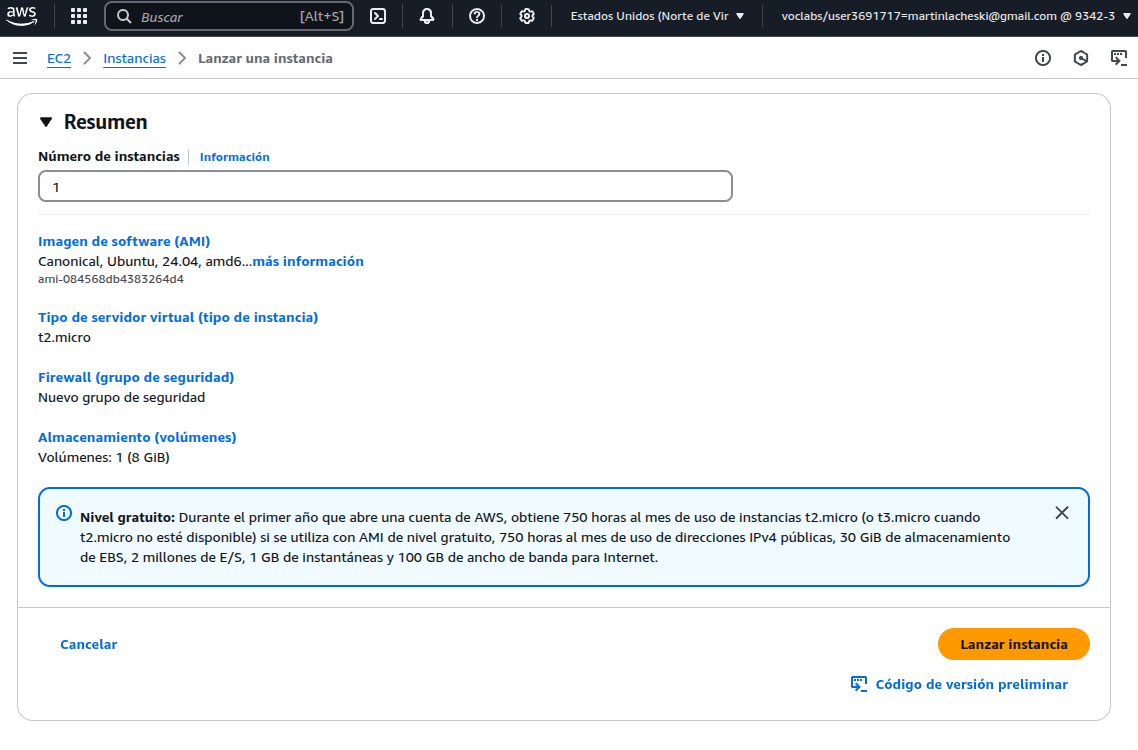
\includegraphics[width=\textwidth]{./Images/32-ec2-1.png}
    \caption{Resumen de la instancia EC2 creada.}
    \label{fig:aws-ec2}
\end{figure}

\section{Instalación y configuración del servidor EC2}

Una vez creada la instancia EC2, se procedió a su configuración e instalación
de los servicios necesarios para el funcionamiento del sistema
\texttt{EnviroSenseIoT}. Para ello, se siguieron los siguientes pasos:

\subsection{Conectarse a la instancia EC2}
Para establecer una conexión con una instancia EC2 mediante SSH, primero se
debe abrir una terminal y ubicar la clave privada
\texttt{envirosense-app-key.pem}, que será utilizada para la autenticación. Es
fundamental restringir los permisos del archivo para que solo el propietario
tenga acceso de lectura, de modo que el sistema SSH lo acepte como válido. Esto
se logra al ejecutar el siguiente comando:

\begin{verbatim}
chmod 400 envirosense-app-key.pem
\end{verbatim}

Una vez configurados los permisos, se puede establecer la conexión al utilizar
el DNS público de la instancia. Por ejemplo:

\begin{verbatim}
ssh -i "key.pem" ubuntu@ec2-X.compute-1.amazonaws.com
\end{verbatim}

La figura \ref{fig:aws-ec2-ssh} muestra la conexión SSH a la instancia EC2.
\begin{figure}[H]
    \centering
    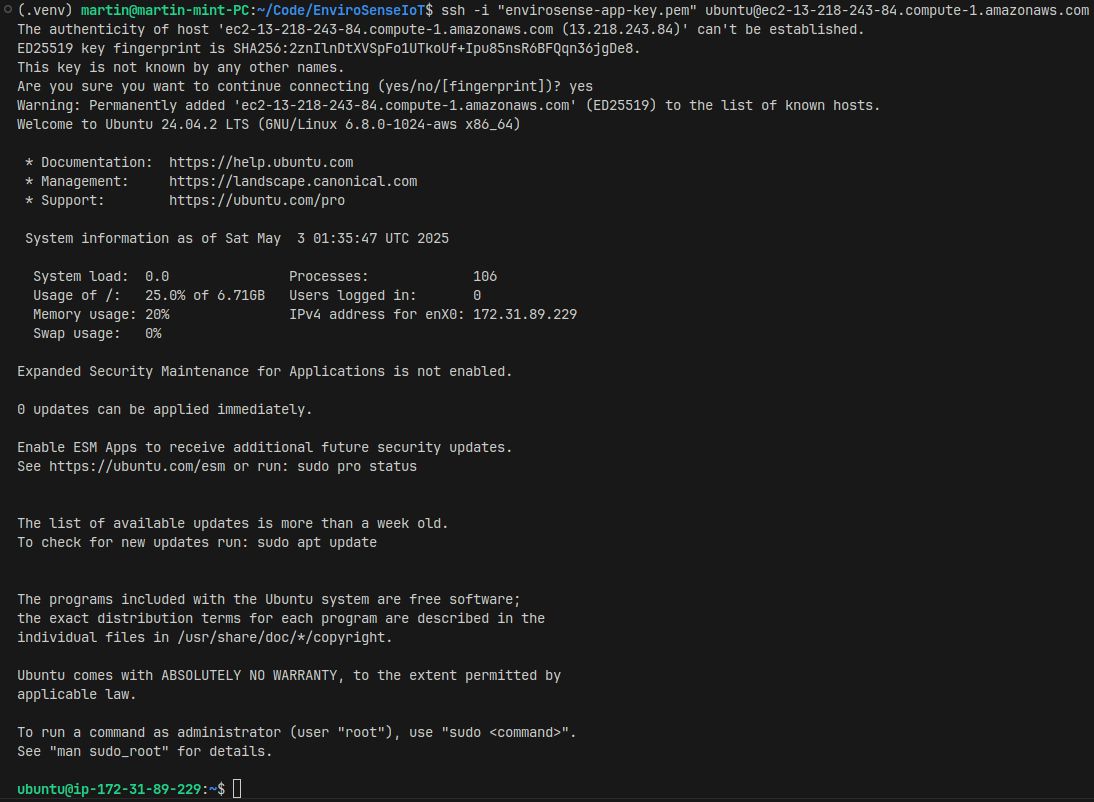
\includegraphics[width=\textwidth]{./Images/33-ec2-2.png}
    \caption{Conexión SSH a la instancia EC2.}
    \label{fig:aws-ec2-ssh}
\end{figure}

Una vez que se ingresó a la instancia EC2, se actualizaron los paquetes del
sistema con los comandos:

\begin{verbatim}
sudo apt update
sudo apt upgrade
\end{verbatim}

\subsection{Instalación de Docker}
Para instalar Docker en Ubuntu, se siguió el tutorial oficial disponible en
\url{https://docs.docker.com/engine/install/ubuntu/}. A continuación, se
detallan los pasos realizados:

En primer lugar, se actualizó el sistema y se instalaron las dependencias
necesarias:

\begin{verbatim}
sudo apt-get update
sudo apt-get install ca-certificates curl
sudo install -m 0755 -d /etc/apt/keyrings
sudo curl -fsSL https://download.docker.com/linux/ubuntu/gpg
 -o /etc/apt/keyrings/docker.asc
sudo chmod a+r /etc/apt/keyrings/docker.asc
\end{verbatim}

Luego, se agregó el repositorio de Docker a las fuentes de APT y se actualizó
nuevamente el sistema:

\begin{verbatim}
echo \
  "deb [arch=$(dpkg --print-architecture) signed-by=/etc/apt
  /keyrings/docker.asc] \
  https://download.docker.com/linux/ubuntu \
  $(. /etc/os-release && 
  echo "${UBUNTU_CODENAME:-$VERSION_CODENAME}") stable" | \
  sudo tee /etc/apt/sources.list.d/docker.list > /dev/null
sudo apt-get update
\end{verbatim}

A continuación, se procedió a instalar Docker y sus componentes esenciales, y
se verificó la instalación mediante los siguientes comandos:

\begin{verbatim}
sudo apt-get install docker-ce docker-ce-cli containerd.io 
 docker-buildx-plugin docker-compose-plugin
sudo docker run hello-world
\end{verbatim}

Para permitir el uso de Docker sin la necesidad de utilizar \texttt{sudo}, se
agregó el usuario al grupo \texttt{docker} con los siguientes comandos:

\begin{verbatim}
sudo groupadd docker
sudo usermod -aG docker $USER
newgrp docker
docker run hello-world
\end{verbatim}

Por último, se configuraron los servicios de Docker y containerd para que se
inicien automáticamente al arrancar el sistema, mediante los siguientes
comandos:

\begin{verbatim}
sudo systemctl enable docker.service
sudo systemctl enable containerd.service
\end{verbatim}

\subsection{Instalación de Docker Compose}

Para instalar Docker Compose, se siguieron los siguientes pasos: Se descargó la
versión más reciente de Docker Compose desde el repositorio oficial de GitHub.
En este caso, se utilizó la versión 2.17.2, que es la última versión estable al
momento de la instalación. Se utilizó el siguiente comando para descargar el
binario de Docker Compose y guardarlo en la ruta
\texttt{/usr/local/bin/docker-compose}:
\begin{verbatim}
sudo curl -SL
 https://github.com/docker/compose/releases/download/
 v2.17.2/docker-compose-linux-x86_64 
 -o /usr/local/bin/docker-compose
\end{verbatim}

Luego, se asignaron permisos de ejecución al binario de Docker Compose para que
pueda ser ejecutado con el siguiente comando:

\begin{verbatim}
sudo chmod +x /usr/local/bin/docker-compose
\end{verbatim}

A continuación, se verificó que la instalación fuera exitosa mediante:

\begin{verbatim}
docker-compose --version
\end{verbatim}

Finalmente, se creó un enlace simbólico para facilitar su ejecución desde
cualquier ruta del sistema:

\begin{verbatim}
sudo ln -s /usr/local/bin/docker-compose 
 /usr/bin/docker-compose
\end{verbatim}

\subsection{Instalación del cliente DuckDNS}

Para comenzar con la instalación del cliente DuckDNS en la instancia EC2, se
instalaron los paquetes necesarios mediante los siguientes comandos:

\begin{verbatim}
sudo apt-get update && sudo apt-get install cloud-utils -y
sudo apt install amazon-ec2-utils
\end{verbatim}

A continuación, se siguieron las instrucciones proporcionadas por el sitio
oficial de DuckDNS, específicamente en la sección para instancias EC2.

Luego, se creó un archivo llamado \texttt{duck.sh} en el directorio raíz del
servidor. Este script se encarga de verificar si la dirección IP pública ha
cambiado y, en caso afirmativo, actualizar el registro correspondiente en
DuckDNS. El contenido del archivo es el siguiente:

\begin{verbatim}
#!/bin/bash
current_ip=""
while true; do
latest_ip=$(ec2-metadata --public-ipv4 | cut -d " " -f 2)
[ -z "$latest_ip" ] && latest_ip=$(curl -s ifconfig.me)
echo "Current IP: $current_ip | Latest IP: $latest_ip"
if [ "$current_ip" == "$latest_ip" ]; then
echo "IP no ha cambiado."
else
echo "IP ha cambiado. Se actualiza DuckDNS..."
current_ip="$latest_ip"
response=$(curl -s -k "https://www.duckdns.org/update?
 domains=envirosense&token=TOKEN&ip=$latest_ip")
echo "DuckDNS response: $response" >> ~/duckdns/duck.log
fi
sleep 5m
done
\end{verbatim}

Este script se ejecuta de forma continua, verifica cada cinco minutos si se
produjo un cambio en la IP pública de la instancia.

\subsection{Descarga y configuración del repositorio EnviroSense}

Para poner en marcha el sistema, primero se clonó el repositorio del código
fuente desde GitHub y se accedió al directorio correspondiente con los
siguientes comandos:

\begin{verbatim}
git clone 
 https://github.com/martinlacheski/EnviroSenseIoT.git
cd EnviroSenseIoT
\end{verbatim}

A continuación, se ingresó al directorio EnviroSenseIoT y se creó el archivo
\texttt{.env}, donde se definieron las variables de entorno necesarias para el
correcto funcionamiento del sistema. Para ello, se utilizó el siguiente
comando:

\begin{verbatim}
nano .env
\end{verbatim}

En este archivo se incluyó la configuración vinculada a la conexión con la base
de datos MongoDB, claves JWT para autenticación, y parámetros específicos tanto
del backend como del frontend.

El contenido del archivo \texttt{.env} tiene los siguientes parámetros:
\begin{verbatim}
# Conexión MongoDB
MONGO_HOST=host # Dirección IP o nombre de host de MongoDB
MONGO_USER=user # Nombre de usuario para la conexión
MONGO_PASSWORD=password # Contraseña para la conexión
MONGO_DB=database # Nombre de la base de datos
    
# Conexión Backend
BACKEND_HOST=0.0.0.0 # Permitir conexión desde cualquier IP
BACKEND_CORS_ORIGINS=origins # Orígenes permitidos
    
# Configuración de JWT
# Generar una clave secreta con el comando: 
# openssl rand -hex 32
BACKEND_SECRET_KEY=clave # Clave secreta generada
BACKEND_ALGORITHM="HS256" # Algoritmo de firma
BACKEND_ACCESS_TOKEN_EXPIRE_MINUTES=120 # Expiración token

# Configuración de Frontend
VITE_PWD_SIGNUP_ENABLED=true
VITE_BACKEND_API_URL=url # URL del backend
VITE_BACKEND_SOCKET_URL=url # URL del socket
\end{verbatim}

Luego, se accedió al directorio \texttt{backend} del proyecto y se creó una
carpeta llamada \texttt{certificates}, destinada a almacenar los certificados
necesarios para las conexiones seguras:

\begin{verbatim}
cd backend
mkdir certificates
\end{verbatim}

Dentro de esta carpeta, se generaron los archivos \texttt{client.crt},
\texttt{client.key} y \texttt{root.crt}, que contienen los certificados y la
clave privada requeridos por AWS IoT Core para establecer comunicaciones
seguras vía MQTT con TLS.

\subsection{Configuración del sistema como servicio}

Para garantizar que la aplicación se inicie automáticamente con el sistema, se
creó un servicio a través de \texttt{systemd}. En primer lugar, se generó el
archivo de configuración del servicio con el siguiente comando:

\begin{verbatim}
sudo nano /etc/systemd/system/envirosense-iot.service
\end{verbatim}

Dentro del archivo, se definió el siguiente contenido:

\begin{verbatim}
[Unit]
Description=EnviroSenseIoT Docker Compose
After=docker.service
Requires=docker.service

[Service]
Type=oneshot
RemainAfterExit=yes
WorkingDirectory=/home/ubuntu/EnviroSenseIoT
ExecStart=/usr/bin/docker-compose up --build -d
ExecStop=/usr/bin/docker-compose down
TimeoutStartSec=0

[Install]
WantedBy=multi-user.target
\end{verbatim}

Este servicio está diseñado para levantar y detener los contenedores Docker
definidos en el archivo \texttt{docker-compose.yml}, ubicado en el directorio
del sistema.

Luego se recargó la configuración de \texttt{systemd} con el siguiente comando:

\begin{verbatim}
sudo systemctl daemon-reload
\end{verbatim}

Luego, se habilitó el servicio para que se ejecute automáticamente al iniciar
el sistema:

\begin{verbatim}
sudo systemctl enable envirosense-iot.service
\end{verbatim}

También se realizó una prueba de ejecución manual del servicio para validar su
funcionamiento:

\begin{verbatim}
sudo systemctl start envirosense-iot.service
\end{verbatim}

Para comprobar que la aplicación se ejecutaba correctamente, se consultó el
estado del servicio y se verificó la actividad de los contenedores:

\begin{verbatim}
sudo systemctl status envirosense-iot.service
docker ps
\end{verbatim}

Finalmente, se realizó un reinicio del sistema para asegurarse de que el
servicio se active correctamente de forma automática:

\begin{verbatim}
sudo reboot now
\end{verbatim}

Después del reinicio, se validó que los contenedores estuvieran en ejecución y
que el servicio estuviera activo:

\begin{verbatim}
docker ps
sudo systemctl status envirosense-iot.service
\end{verbatim}

La figura \ref{fig:aws-ec2-service} muestra el acceso a la aplicación web
\texttt{EnviroSenseIoT} a través del navegador web, con el nombre de dominio
\texttt{envirosense.duckdns.org} asociado a la IP pública de la instancia EC2.
\begin{figure}[H]
    \centering
    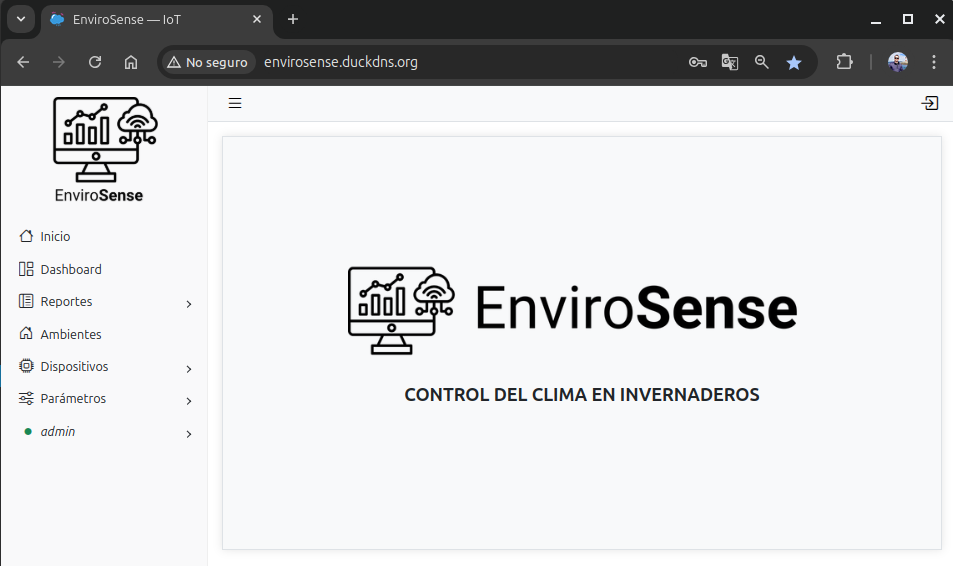
\includegraphics[width=\textwidth]{./Images/34-ec2-3.png}
    \caption{Acceso a la aplicación web EnviroSenseIoT.}
    \label{fig:aws-ec2-service}
\end{figure}

Finalmente, se comprobó el correcto funcionamiento de la aplicación y la
comunicación mediante WebSocket, lo que permitió visualizar los datos en tiempo
real. La figura \ref{fig:aws-ec2-websocket} ilustra cómo se presentan estos
datos en la interfaz web desplegada en la instancia EC2.

\begin{figure}[H]
    \centering
    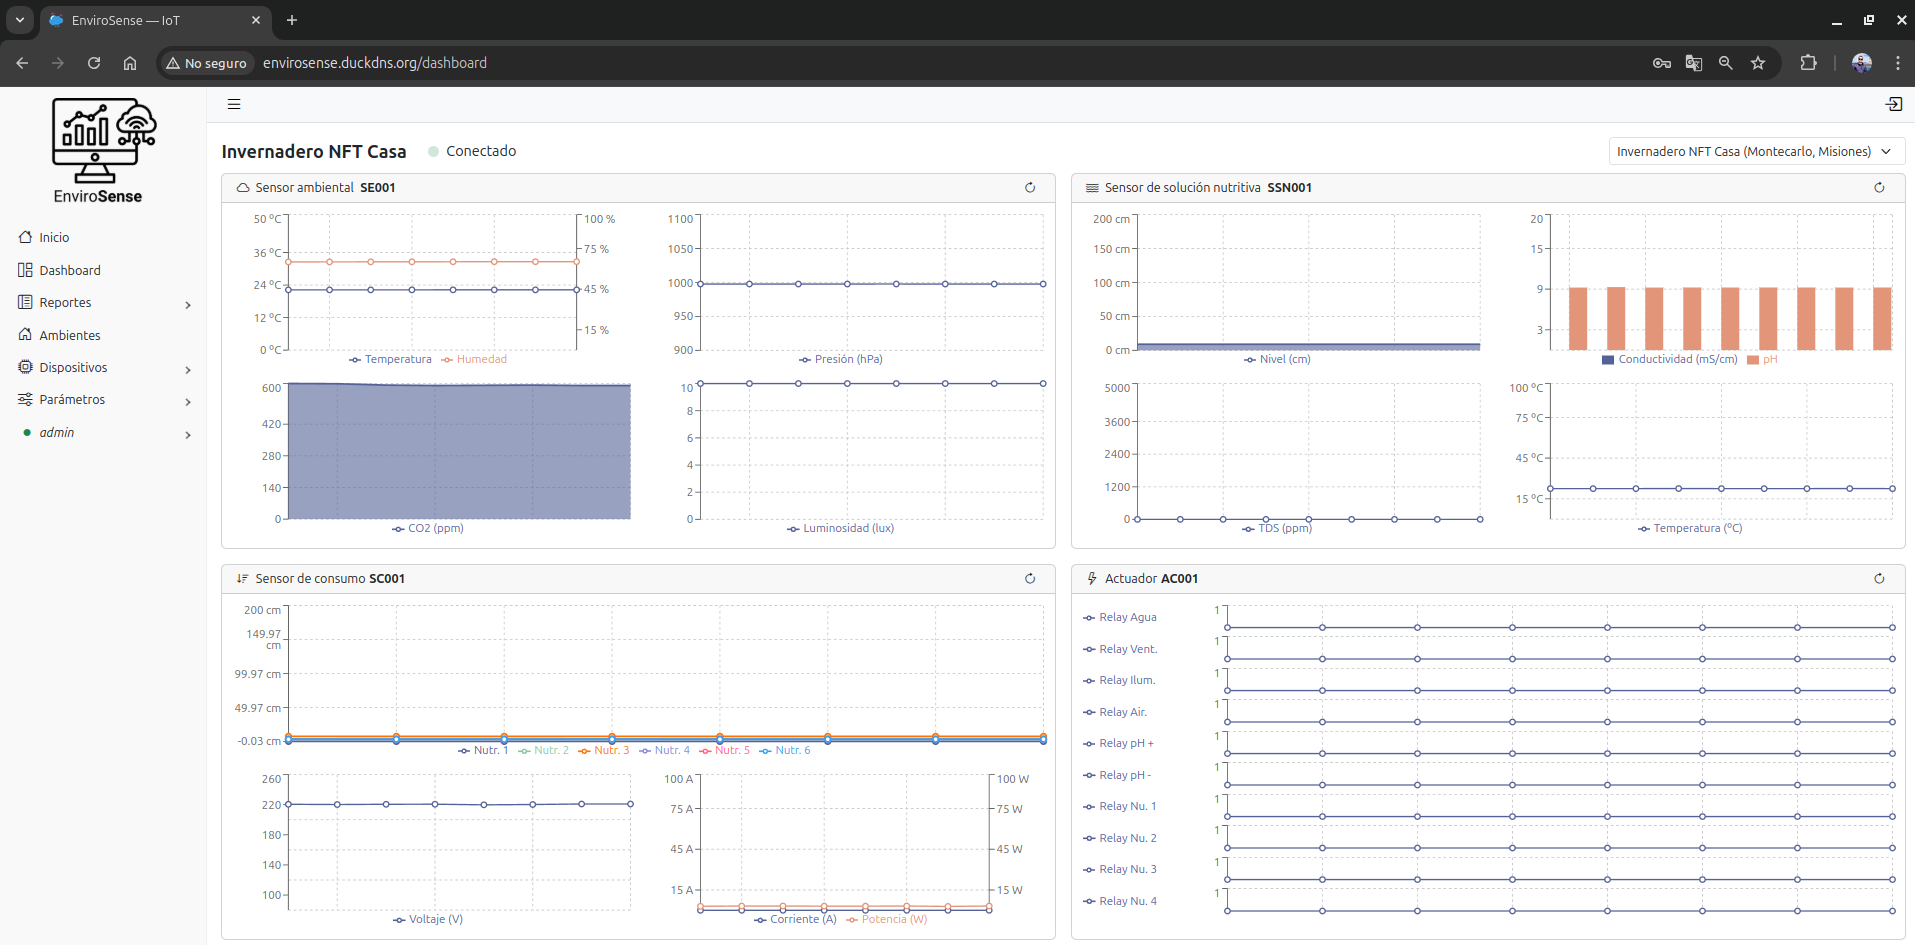
\includegraphics[width=\textwidth]{./Images/35-ec2-4.png}
    \caption{Visualización de datos en tiempo real.}
    \label{fig:aws-ec2-websocket}
\end{figure}

